% GNUPLOT: LaTeX picture with Postscript
\begingroup
  \makeatletter
  \providecommand\color[2][]{%
    \GenericError{(gnuplot) \space\space\space\@spaces}{%
      Package color not loaded in conjunction with
      terminal option `colourtext'%
    }{See the gnuplot documentation for explanation.%
    }{Either use 'blacktext' in gnuplot or load the package
      color.sty in LaTeX.}%
    \renewcommand\color[2][]{}%
  }%
  \providecommand\includegraphics[2][]{%
    \GenericError{(gnuplot) \space\space\space\@spaces}{%
      Package graphicx or graphics not loaded%
    }{See the gnuplot documentation for explanation.%
    }{The gnuplot epslatex terminal needs graphicx.sty or graphics.sty.}%
    \renewcommand\includegraphics[2][]{}%
  }%
  \providecommand\rotatebox[2]{#2}%
  \@ifundefined{ifGPcolor}{%
    \newif\ifGPcolor
    \GPcolortrue
  }{}%
  \@ifundefined{ifGPblacktext}{%
    \newif\ifGPblacktext
    \GPblacktexttrue
  }{}%
  % define a \g@addto@macro without @ in the name:
  \let\gplgaddtomacro\g@addto@macro
  % define empty templates for all commands taking text:
  \gdef\gplbacktext{}%
  \gdef\gplfronttext{}%
  \makeatother
  \ifGPblacktext
    % no textcolor at all
    \def\colorrgb#1{}%
    \def\colorgray#1{}%
  \else
    % gray or color?
    \ifGPcolor
      \def\colorrgb#1{\color[rgb]{#1}}%
      \def\colorgray#1{\color[gray]{#1}}%
      \expandafter\def\csname LTw\endcsname{\color{white}}%
      \expandafter\def\csname LTb\endcsname{\color{black}}%
      \expandafter\def\csname LTa\endcsname{\color{black}}%
      \expandafter\def\csname LT0\endcsname{\color[rgb]{1,0,0}}%
      \expandafter\def\csname LT1\endcsname{\color[rgb]{0,1,0}}%
      \expandafter\def\csname LT2\endcsname{\color[rgb]{0,0,1}}%
      \expandafter\def\csname LT3\endcsname{\color[rgb]{1,0,1}}%
      \expandafter\def\csname LT4\endcsname{\color[rgb]{0,1,1}}%
      \expandafter\def\csname LT5\endcsname{\color[rgb]{1,1,0}}%
      \expandafter\def\csname LT6\endcsname{\color[rgb]{0,0,0}}%
      \expandafter\def\csname LT7\endcsname{\color[rgb]{1,0.3,0}}%
      \expandafter\def\csname LT8\endcsname{\color[rgb]{0.5,0.5,0.5}}%
    \else
      % gray
      \def\colorrgb#1{\color{black}}%
      \def\colorgray#1{\color[gray]{#1}}%
      \expandafter\def\csname LTw\endcsname{\color{white}}%
      \expandafter\def\csname LTb\endcsname{\color{black}}%
      \expandafter\def\csname LTa\endcsname{\color{black}}%
      \expandafter\def\csname LT0\endcsname{\color{black}}%
      \expandafter\def\csname LT1\endcsname{\color{black}}%
      \expandafter\def\csname LT2\endcsname{\color{black}}%
      \expandafter\def\csname LT3\endcsname{\color{black}}%
      \expandafter\def\csname LT4\endcsname{\color{black}}%
      \expandafter\def\csname LT5\endcsname{\color{black}}%
      \expandafter\def\csname LT6\endcsname{\color{black}}%
      \expandafter\def\csname LT7\endcsname{\color{black}}%
      \expandafter\def\csname LT8\endcsname{\color{black}}%
    \fi
  \fi
    \setlength{\unitlength}{0.0500bp}%
    \ifx\gptboxheight\undefined%
      \newlength{\gptboxheight}%
      \newlength{\gptboxwidth}%
      \newsavebox{\gptboxtext}%
    \fi%
    \setlength{\fboxrule}{0.5pt}%
    \setlength{\fboxsep}{1pt}%
    \definecolor{tbcol}{rgb}{1,1,1}%
\begin{picture}(3740.00,4020.00)%
    \gplgaddtomacro\gplbacktext{%
      \csname LTb\endcsname%%
      \put(373,699){\makebox(0,0)[r]{\strut{}$-150$}}%
      \csname LTb\endcsname%%
      \put(373,1133){\makebox(0,0)[r]{\strut{}$-100$}}%
      \csname LTb\endcsname%%
      \put(373,1566){\makebox(0,0)[r]{\strut{}$-50$}}%
      \csname LTb\endcsname%%
      \put(373,2000){\makebox(0,0)[r]{\strut{}$0$}}%
      \csname LTb\endcsname%%
      \put(373,2433){\makebox(0,0)[r]{\strut{}$50$}}%
      \csname LTb\endcsname%%
      \put(373,2866){\makebox(0,0)[r]{\strut{}$100$}}%
      \csname LTb\endcsname%%
      \put(373,3300){\makebox(0,0)[r]{\strut{}$150$}}%
      \csname LTb\endcsname%%
      \put(731,263){\makebox(0,0){\strut{}$-150$}}%
      \csname LTb\endcsname%%
      \put(1164,263){\makebox(0,0){\strut{}$-100$}}%
      \csname LTb\endcsname%%
      \put(1597,263){\makebox(0,0){\strut{}$-50$}}%
      \csname LTb\endcsname%%
      \put(2031,263){\makebox(0,0){\strut{}$0$}}%
      \csname LTb\endcsname%%
      \put(2464,263){\makebox(0,0){\strut{}$50$}}%
      \csname LTb\endcsname%%
      \put(2898,263){\makebox(0,0){\strut{}$100$}}%
      \csname LTb\endcsname%%
      \put(3331,263){\makebox(0,0){\strut{}$150$}}%
    }%
    \gplgaddtomacro\gplfronttext{%
      \csname LTb\endcsname%%
      \put(16,1999){\rotatebox{-270.00}{\makebox(0,0){\normalsize $\Psi$}}}%
      \csname LTb\endcsname%%
      \put(2031,0){\makebox(0,0){\normalsize $\Phi$}}%
      \csname LTb\endcsname%%
      \put(1920,2196){\rotatebox{150.00}{\makebox(0,0){\strut{}\textcolor{black}{\footnotesize 1.3}}}}%
      \csname LTb\endcsname%%
      \put(1826,1862){\rotatebox{-57.00}{\makebox(0,0){\strut{}\textcolor{black}{\footnotesize 1.4}}}}%
      \csname LTb\endcsname%%
      \put(2330,2257){\rotatebox{124.00}{\makebox(0,0){\strut{}\textcolor{black}{\footnotesize 1.5}}}}%
      \csname LTb\endcsname%%
      \put(2015,1441){\rotatebox{-36.00}{\makebox(0,0){\strut{}\textcolor{black}{\footnotesize 1.5}}}}%
      \csname LTb\endcsname%%
      \put(1655,2803){\rotatebox{51.00}{\makebox(0,0){\strut{}\textcolor{black}{\footnotesize 1.6}}}}%
      \csname LTb\endcsname%%
      \put(1743,1290){\rotatebox{-79.00}{\makebox(0,0){\strut{}\textcolor{black}{\footnotesize 1.6}}}}%
      \csname LTb\endcsname%%
      \put(2740,2311){\rotatebox{-15.00}{\makebox(0,0){\strut{}\textcolor{black}{\footnotesize 1.6}}}}%
      \csname LTb\endcsname%%
      \put(2815,1606){\rotatebox{40.00}{\makebox(0,0){\strut{}\textcolor{black}{\footnotesize 1.6}}}}%
      \csname LTb\endcsname%%
      \put(1468,1133){\rotatebox{-81.00}{\makebox(0,0){\strut{}\textcolor{black}{\footnotesize 1.7}}}}%
      \csname LTb\endcsname%%
      \put(1421,2898){\rotatebox{49.00}{\makebox(0,0){\strut{}\textcolor{black}{\footnotesize 1.7}}}}%
      \csname LTb\endcsname%%
      \put(2771,2599){\rotatebox{-26.00}{\makebox(0,0){\strut{}\textcolor{black}{\footnotesize 1.7}}}}%
      \csname LTb\endcsname%%
      \put(2863,1322){\rotatebox{55.00}{\makebox(0,0){\strut{}\textcolor{black}{\footnotesize 1.7}}}}%
      \csname LTb\endcsname%%
      \put(2031,3823){\makebox(0,0){VBA EA (eV)}}%
    }%
    \gplbacktext
    \put(0,0){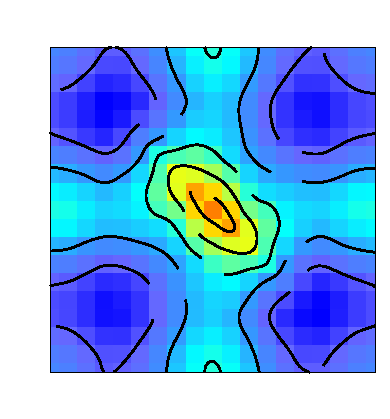
\includegraphics[width={187.00bp},height={201.00bp}]{Q0_VBA}}%
    \gplfronttext
  \end{picture}%
\endgroup
